\documentclass[11pt,oneside]{article}
\usepackage[T1]{fontenc}
\usepackage{amsmath,amsthm,amssymb}
\usepackage{mathpazo}
\usepackage{amsfonts,bm}

\usepackage{hyperref}

\hypersetup{
  colorlinks,
  linkcolor=blue
}

\usepackage{graphicx}
\graphicspath{{../output/}}

\usepackage[letterpaper,
            left=1in,
            right=1in,
            top=1in,
            bottom=1in,
            footskip=.5in]{geometry}

%%%%%%%%%%%%%%%%%%%%%%%%%%%%%%%%COMMANDS%%%%%%%%%%%%%%%%%%%%%%%%%%%%%%%%

\newcommand{\bb}[1]{\textbf{#1}}

\newcommand{\R}{\mathbb{R}}

% vector (always lower case)
\renewcommand{\vec}[1]{
  \ifcat\noexpand#1\relax
    \bm{#1}
  \else
    \mathbf{#1}
  \fi
}

\newcommand{\mat}[1]{
  \ifcat\noexpand#1\relax
    \bm{#1}
  \else
    \mathbf{#1}
  \fi
}

\newcommand{\norm}[1]{\left\lVert#1\right\rVert}

\newcommand{\tr}{\text{Tr}}

\renewcommand{\arraystretch}{1.4} % make rows wider

%%%%%%%%%%%%%%%%%%%%%%%%%%%%%%%%DOCUMENT%%%%%%%%%%%%%%%%%%%%%%%%%%%%%%%%

\begin{document}

{\Large\bf BIOS 611 Final Project}

\smallskip
{\large\bf Spatial transcriptomic data from human breast cancer tissue}

\smallskip
Name: Hongyu Yu\quad PID: 730440679

\section{Introduction}

The human breast cancer spatial transcriptomic data used in this report was from \href{https://www.science.org/doi/10.1126/science.aaf2403}{Ståhl et al, 2016}. The processed data in \texttt{.rds} format was downloaded from \href{https://github.com/xzhoulab/SPARK/blob/master/data/Layer2_BC_Count.rds}{GitHub}, which was uploaded by the authors as a supplementary for a methodology \href{https://www.nature.com/articles/s41592-019-0701-7}{paper} published in Nature Methods. The data contains the gene expression profile of approximately 15,000 genes at about 250 positions in a human breast cancer tissue, and thus each entry represents the number of detected mRNA associated with a gene in a location.

Compared to traditional mRNA sequencing data, which only has mRNA count data for each cell or cell groups, spatial transcriptomic data also contain the information about where each cell or cell group locates in the tissue. This additional dimension allows the analysis of transcription pattern across the tissue. Some questions that were hard to answer using mRNA-seq alone became easy to understand using spatial transcriptomic data.

\section{Results}

\subsection{Expression patterns of highly variable genes}

In a tissue, most genes exhibit similar expression patterns across different cells. These genes can include the house keeping genes, which maintain the basic metabolism of each cell and thus are constantly expressed, or other lowly expressed genes. Since the overall goal is to analyze the expression pattern across the tissue, the main focus is on genes differentially expressed in the experiment. Therefore, the standard deviation of the mRNA count of each gene is calculated and plotted (\autoref{fig:std_genes} left panel). As expected, most genes showed similar expression or were sequenced insufficiently, so the majority has a standard deviation below $5$. The top $10$ variable genes were showed on the right panel of \autoref{fig:std_genes}, which were further visualized across the tissue.

\begin{figure}[ht]
\centering
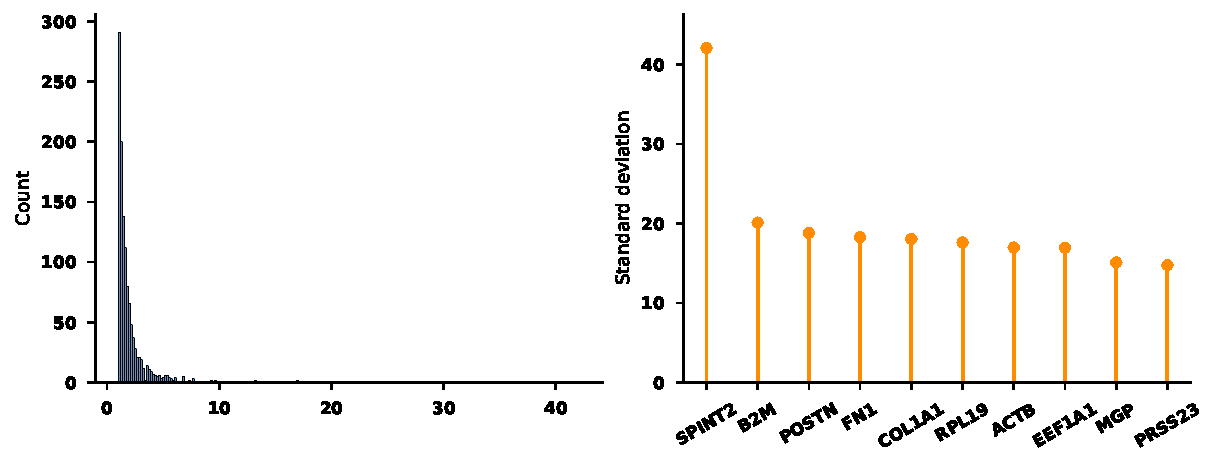
\includegraphics[width=.8\textwidth]{1gene_std.pdf}
\caption{standard deviation of measured  genes}\label{fig:std_genes}
\end{figure}

The expression of highly variable genes is spatially correlated as shown in \autoref{fig:gene_space}. For example, the gene \texttt{COL1A1} is highly expressed in the lower part of the tissue while lowly expressed in other regions. Genes \texttt{FN1} and \texttt{POSTN} also show similar trend. In contrast, \texttt{SPINT2} is only expressed on the left and right corner of the tissue but lowly expressed in the middle part. These together show that gene expression is related to the spatial locations of cells, and different genes have different expression patterns.

\begin{figure}[ht]
\centering
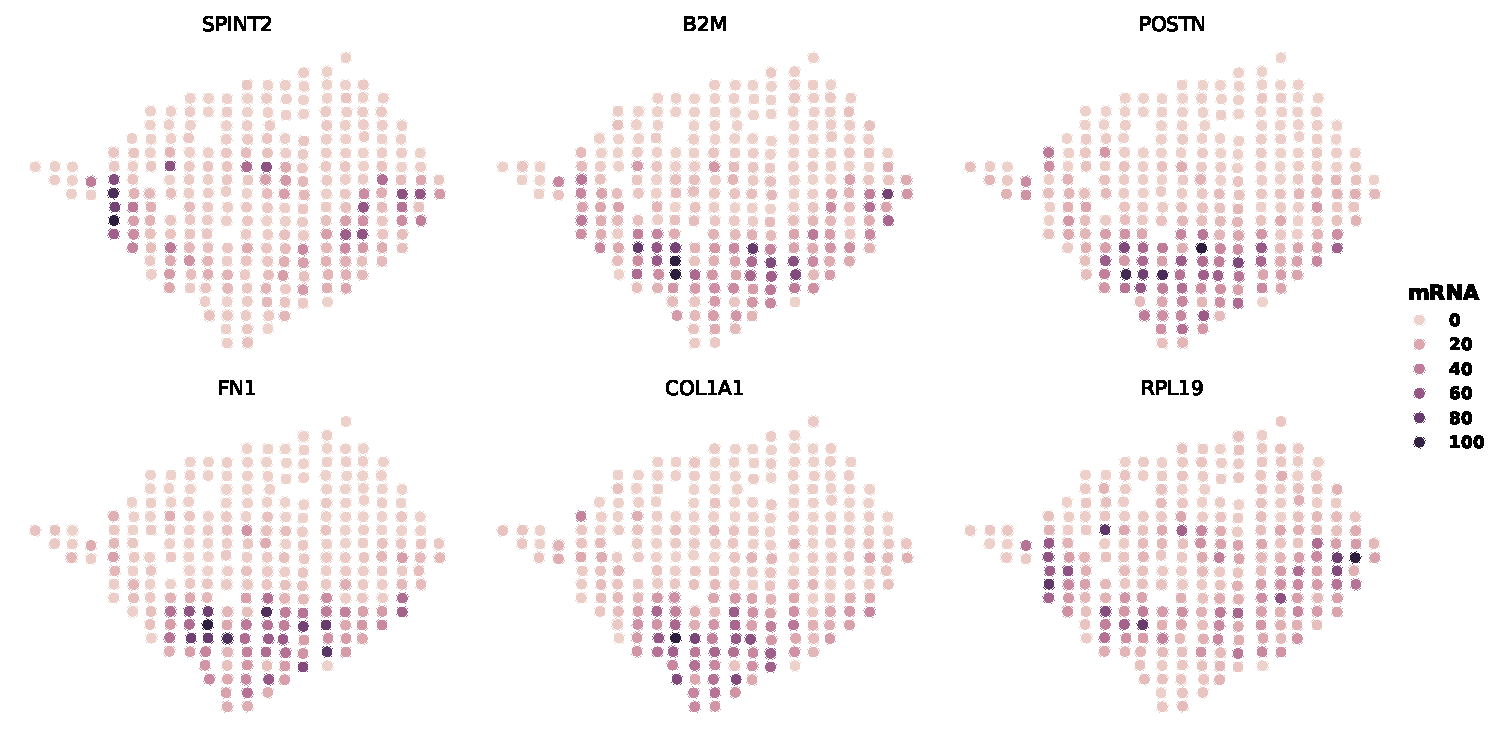
\includegraphics[width=.9\textwidth]{1gene_space.pdf}
\caption{expression of genes across the tissue}
\label{fig:gene_space}
\end{figure}

\subsection{Confounding of gene expression}

The expression pattern observed in the previous section might be attributed to the variation of cell activity across the tissue, but it might also be due to the different sequencing depth at each location. To investigate this potential confounding, the mean expression count of low-variation genes (genes with standard deviation smaller than $5$ across the tissue), is plotted. If all the locations were sequenced similarly well, the mean expression count is expected to be about the same across the entire tissue. However, as shown in \autoref{fig:mean_count}, the mean count is not uniform.

\begin{figure}[ht]
\centering
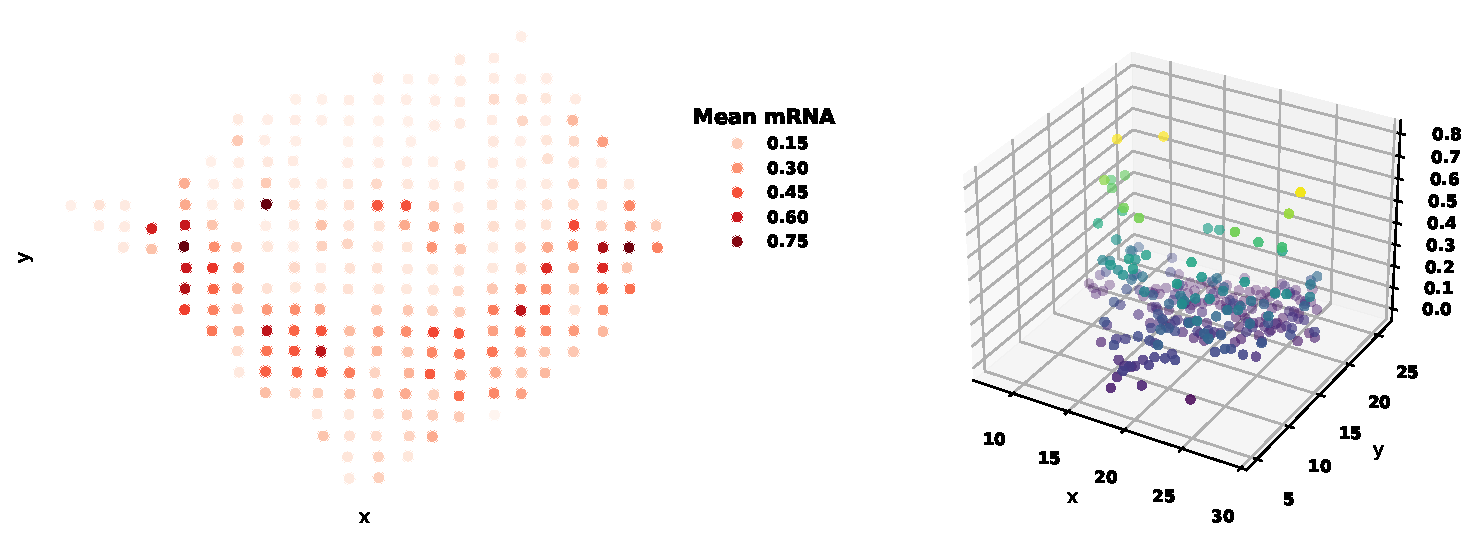
\includegraphics[width=.9\textwidth]{2mean_count.pdf}
\caption{mean expression of low variation genes}
\label{fig:mean_count}
\end{figure}

To examine how the mean expression count affects the expression pattern, the mRNA count at each location for each gene is divided by the average. The mean count of low variation genes is $1$ after normalization (\autoref{fig:mean_count_norm}).

\begin{figure}[ht]
\centering
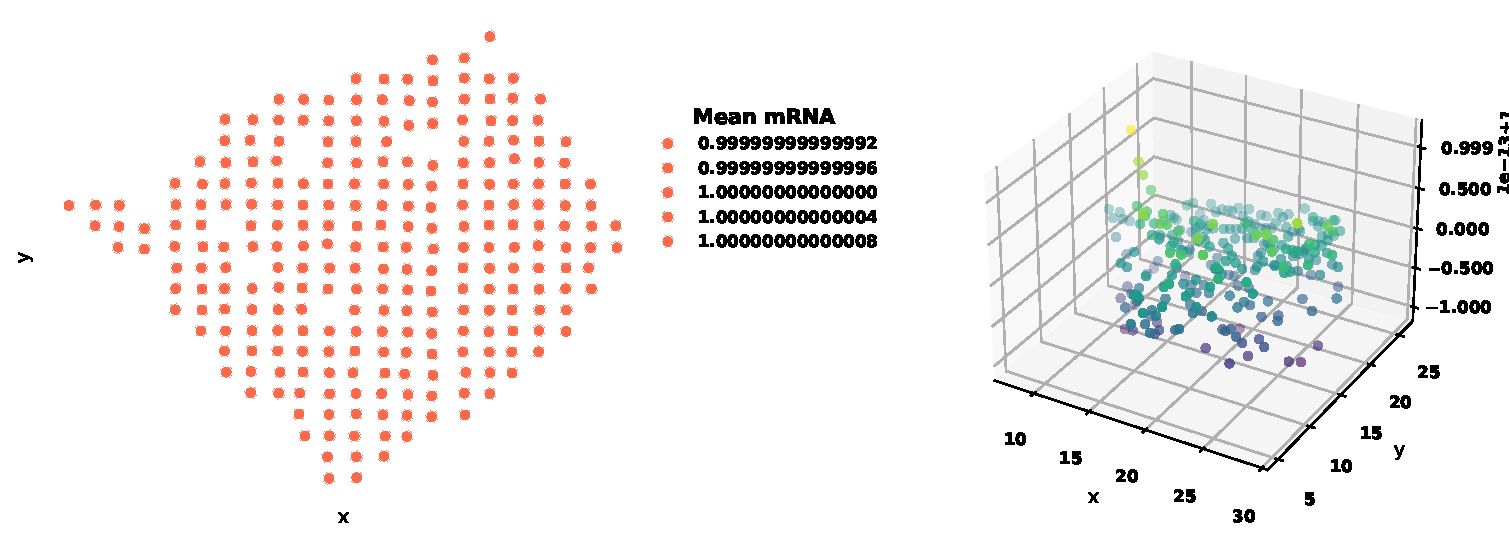
\includegraphics[width=.9\textwidth]{2mean_count_norm.pdf}
\caption{mean expression of low variation genes after normalization}
\label{fig:mean_count_norm}
\end{figure}

The expression patterns of highly variable genes also change as shown in \autoref{fig:gene_space_norm}. For example, \texttt{SPINT2} previously has expression concentrated in the left and the right edge of the tissue while it now has a nearly uniform expression in the entire region. However, the normalization did not remove all the differential expression patterns observed. For \texttt{FN1} and \texttt{COL1A1}, the expression profiles became more concentrated near the bottom of the region (\autoref{fig:gene_space_norm}).

\begin{figure}[ht]
\centering
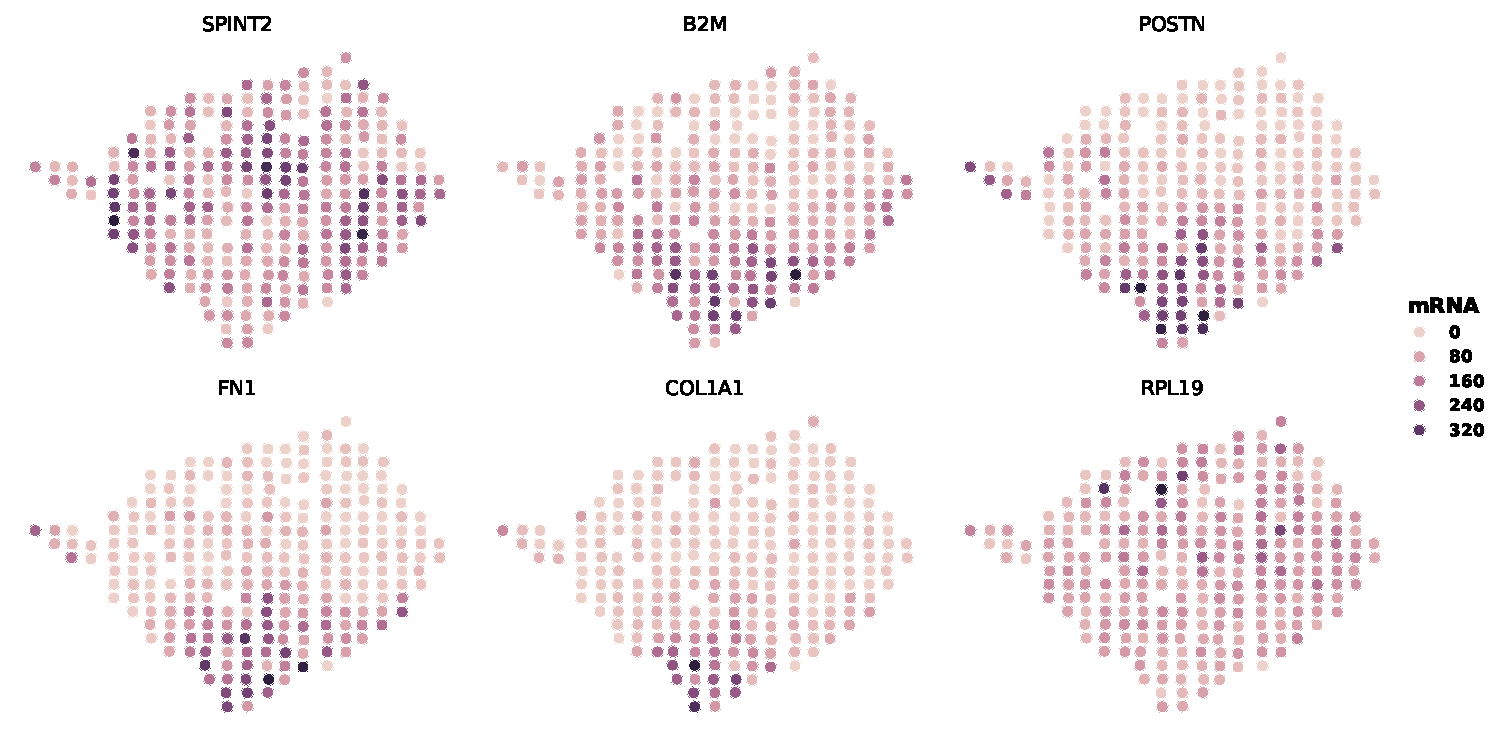
\includegraphics[width=.9\textwidth]{2gene_space_norm.pdf}
\caption{normalized expression of genes across the tissue}
\label{fig:gene_space_norm}
\end{figure}

\subsection{Dimension reduction and clustering}

Another important task in spatial transcriptomics is to identify spatial domains, regions with distinct functions and microenvironments. This can be viewed as a clustering task. Due to the high-dimensionality of transcriptomic data (large number of genes sequenced compared to the number of cells or cell groups), the expression profile are rarely used directly for clustering. Instead, they are first projected to a lower dimensional space, and then clustering is performed on this low dimensional embedding.

In this section, two different dimension reduction methods were tested. The first is a usual PCA, formulated in its variational form as
\begin{equation*}
\min_{\mat Z, \mat W}\norm{\mat X - \mat Z\mat W^\top}_2^2\quad\text{s.t.}\quad \mat W^\top\mat W = \mat I,
\end{equation*}
where $\mat X \in \R^{n\times p}$ is the gene expression data at each location with $X_{ij}$ being the mRNA count of the $j$th gene in the $i$th cell, $\mat W \in \R^{k\times p}$ is an orthognal eigenvector matrix, and $\mat Z \in \R^{n\times k}$ is the $k$-dimensional embedding of all $n$ cells. Write $\mat X = \mat U\mat\Sigma\mat V^\top$. The solution is $\mat Z = \mat U_k\mat \Sigma_k$ and $\mat W = \mat V_k$, where $\mat U_k$ and $\mat V_k$ represent the first $k$ left and right singular vectors and $\mat \Sigma_k$ denote a $k\times k$ diagonal matrix with diagonal elements being the largest $k$ singular values.

The embedding and clustering result of PCA is shown in \autoref{fig:pca_gpca_compare}, left panel. The bottom region of the tissue is identified as one cluster, coherent with previous observations that some highly variable genes show clustered expression at the bottom.

Another dimension reduction method is the \texttt{GraphPCA} proposed in a Genome Biology \href{https://genomebiology.biomedcentral.com/articles/10.1186/s13059-024-03429-x}{paper}. To incorporate the spatial dependency observed in typical spatial transcriptomic data, \texttt{GraphPCA} includes an additional adjancency penalty into PCA. The optimization problem is
\begin{equation*}
\min_{\mat Z, \mat W} \norm{\mat X - \mat Z\mat W^\top}_2^2 + \lambda\tr(\mat Z^\top\mat L\mat Z)\quad\text{s.t.}\quad \mat W^\top\mat W = \mat I,
\end{equation*}
where $\mat L$ is the Graph Laplacian defined by $\mat L = \mat D - \mat A$, where $\mat D$ is the degree of each nodes and $\mat A$ is the adjacency matrix of a graph. The graph used here is a $k$-NN graph, which, for each spatial location, identifies the nearest $k$-locations and connect them as neighbors.

Like PCA, \texttt{GraphPCA} has closed form solution. First, it can be shown that the solution $\mat Z = \mat K\mat X\mat W$, where $\mat K = (\mat I - \lambda \mat L)^{-1}$. Then the problem reduces to
\begin{equation*}
\min_{\mat W}\tr(-\mat W^\top\mat X^\top\mat K\mat X\mat W)\quad\text{s.t.}\quad \mat W^\top\mat W = \mat I,
\end{equation*}
which gives that $\mat W = \mat V_k$, where $\mat V_k$ is the $k$ eigenvectors of $\mat X^\top\mat K\mat X$ associated with the largest $k$ eigenvalues. Therefore, the embedding is $\mat Z = \mat K\mat X\mat V_k$.

\begin{figure}[ht]
\centering
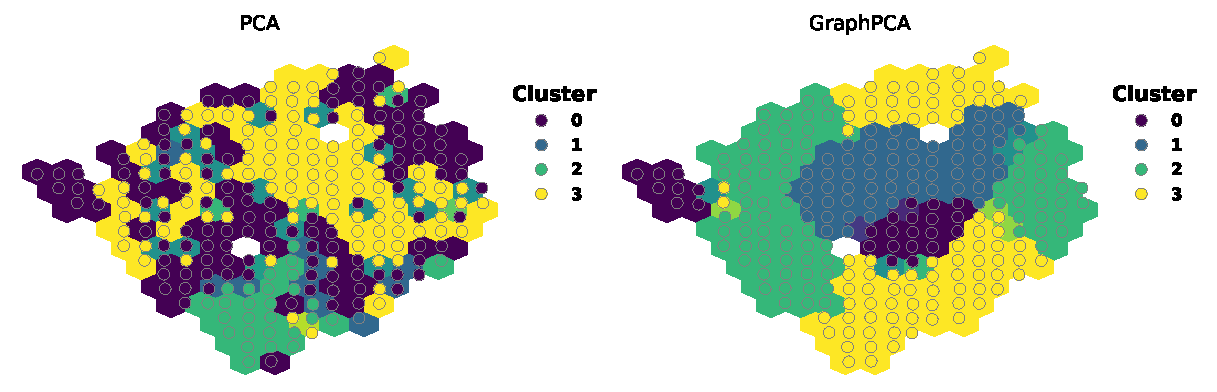
\includegraphics[width=.9\textwidth]{3pca_gpca_compare.pdf}
\caption{clustering based on PCA and GraphPCA}
\label{fig:pca_gpca_compare}
\end{figure}

The \texttt{GraphPCA} clustering result is shown in the right panel of \autoref{fig:pca_gpca_compare}. The $\lambda$ (Graph Laplacian penalization coefficient) and $k$ (number of neighbors) are set as $3$ and $5$, respectively. As expected, \texttt{GraphPCA} yields more spatially continuous clusters compared to plain PCA.

However, a limitation of \texttt{GraphPCA} is that the user has to identify the hyperparameters $\lambda$ and $k$, and as shown in \autoref{gpca_params}. As the penalty term increases, a stronger spatial correlation is expected in the final clustering result though the specific effect also depends on $k$, the number of neighbors in the $k$-NN graph constructed.

\begin{figure}[ht]
\centering
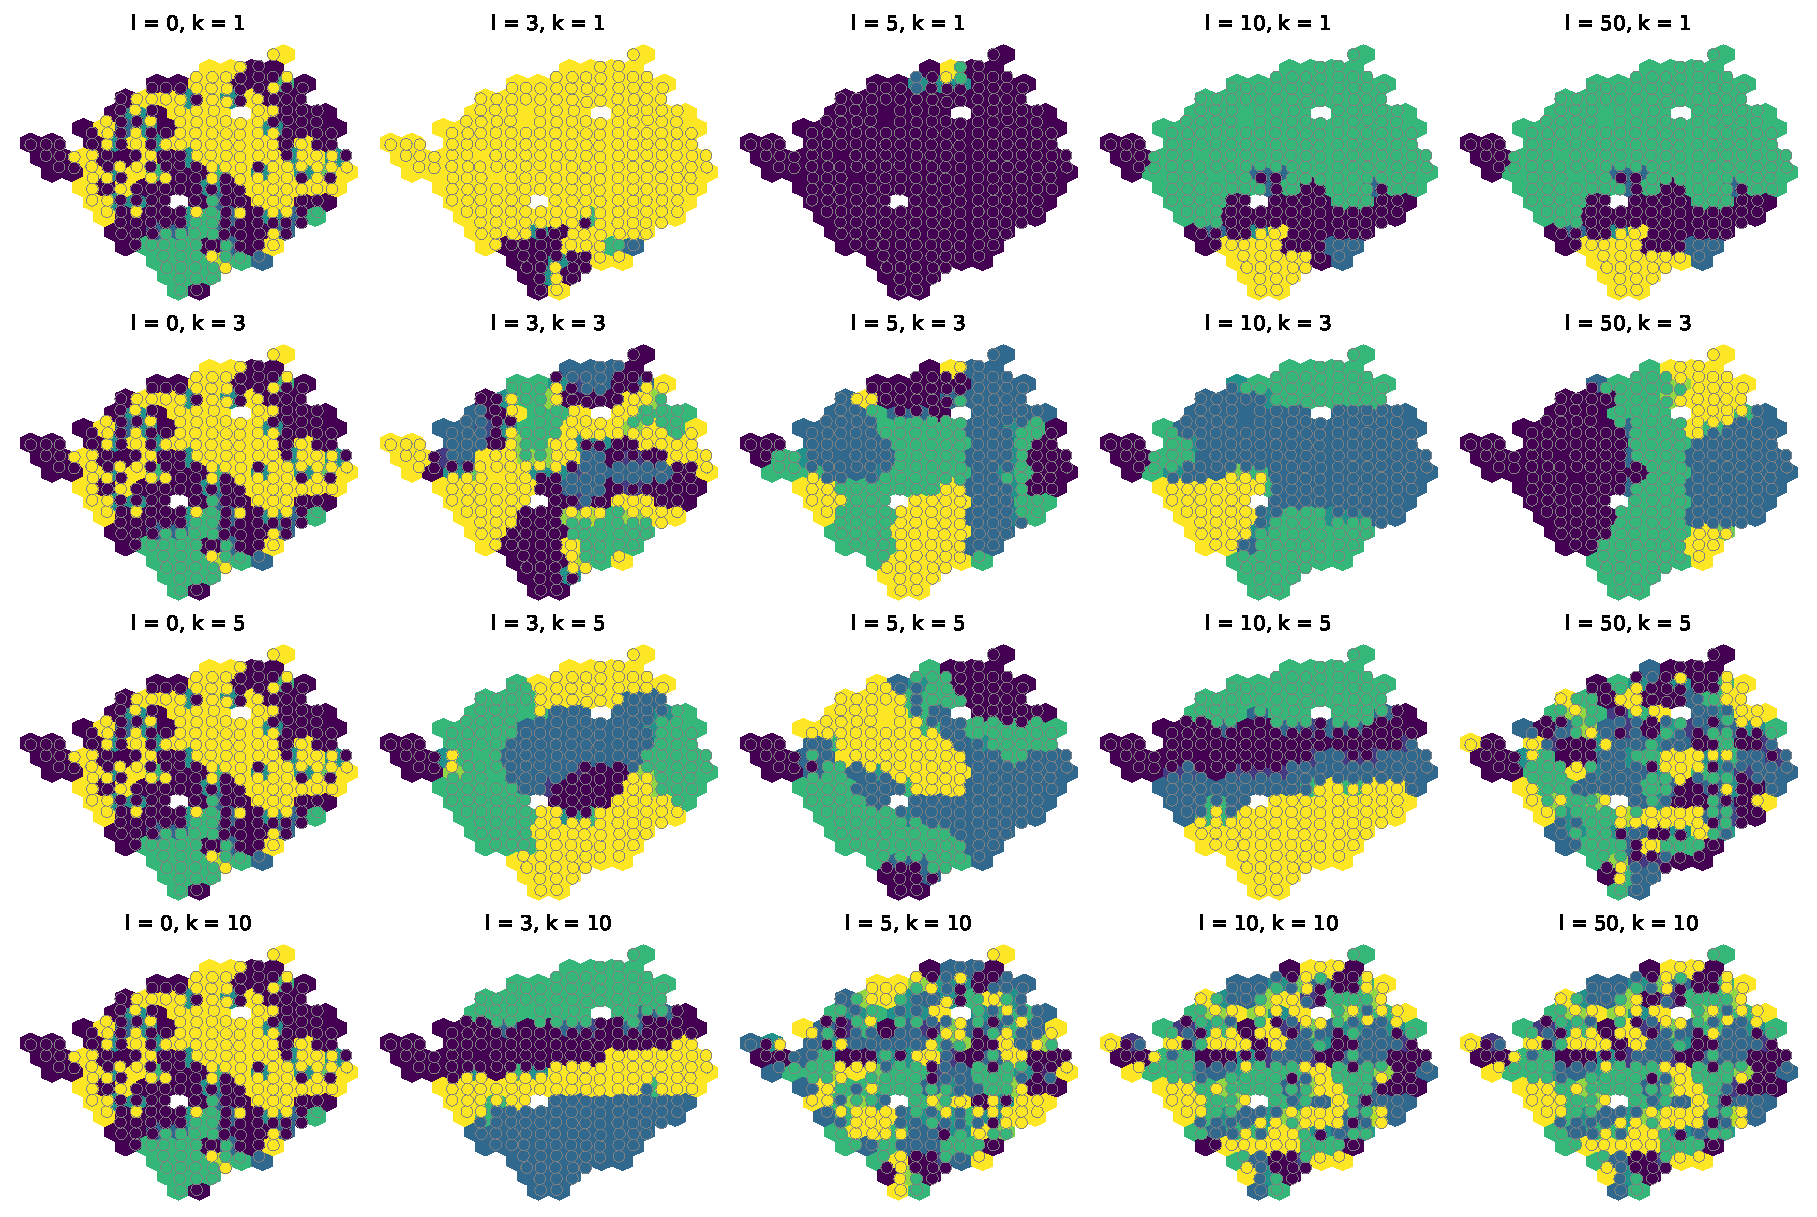
\includegraphics[width=.9\textwidth]{3gpca_params.pdf}
\caption{effects of different values of hyperparameters}
\label{gpca_params}
\end{figure}

\section{Conclusion}

In this report, the spatial transcriptomic data of human breast cancer is re-analyzed. In summary, highly variable genes show distinct expression patterns across the tissue, but the difference in sequencing depth at each spatial location also affects the pattern observed. In addition, clustering results based on PCA and \texttt{GraphPCA} are presented. Though \texttt{GraphPCA} better captures the spatial dependency, it is sensitive to the choice of hyperparameters.

\end{document}